%% ITEM 0 TYPE Frame
\begin{frame}
\frametitle{Table of Contents}
\tableofcontents
\end{frame}
%% ITEM 1 TYPE Section
\section{Caltech student traditions}
%% ITEM 2 TYPE Frame
\begin{frame}
\frametitle{Millikan pumpkin-drop experiment}
Every Halloween, Dabney House conducts the infamous ``Millikan pumpkin-drop experiment'' from the top of Millikan Library, the highest point on campus.

\begin{itemize}
    \item<1-> A claim was once made that the shattering of a pumpkin frozen in liquid nitrogen and dropped from a sufficient height would produce a triboluminescent spark. 
    \item<2-> This yearly event involves a crowd of observers, who try to spot the elusive spark.
    \item<3-> The title of the event is an oblique reference to the famous Millikan oil-drop experiment which measured $e$, the elemental unit of electrical charge.
\end{itemize}

\end{frame}
%% ITEM 3 TYPE Frame
\begin{frame}  
This slide is to test mathematical formulas

$$E=mc^2$$ 

as well as the ``pause'' functionality
\end{frame}
%% ITEM 4 TYPE Section
\section{Caltech student pranks}
%% ITEM 5 TYPE Frame
\begin{frame}
\frametitle{Caltech student pranks}

This is a brief introduction of \alert{Caltech pranks}.

\begin{block}{Definition}
Prank: a practical joke or mischievous act
\end{block}

\begin{alertblock}{Axiom}
Caltech pranks are a key part of the institute's history and identity.
\end{alertblock}

\begin{examples}
See the next slide for a prank example.
\end{examples}
\end{frame}
%% ITEM 6 TYPE Frame
\begin{frame}
\frametitle{Hollywood sign}

\begin{columns}

\column{0.45\textwidth}

\begin{figure}
    \centering
    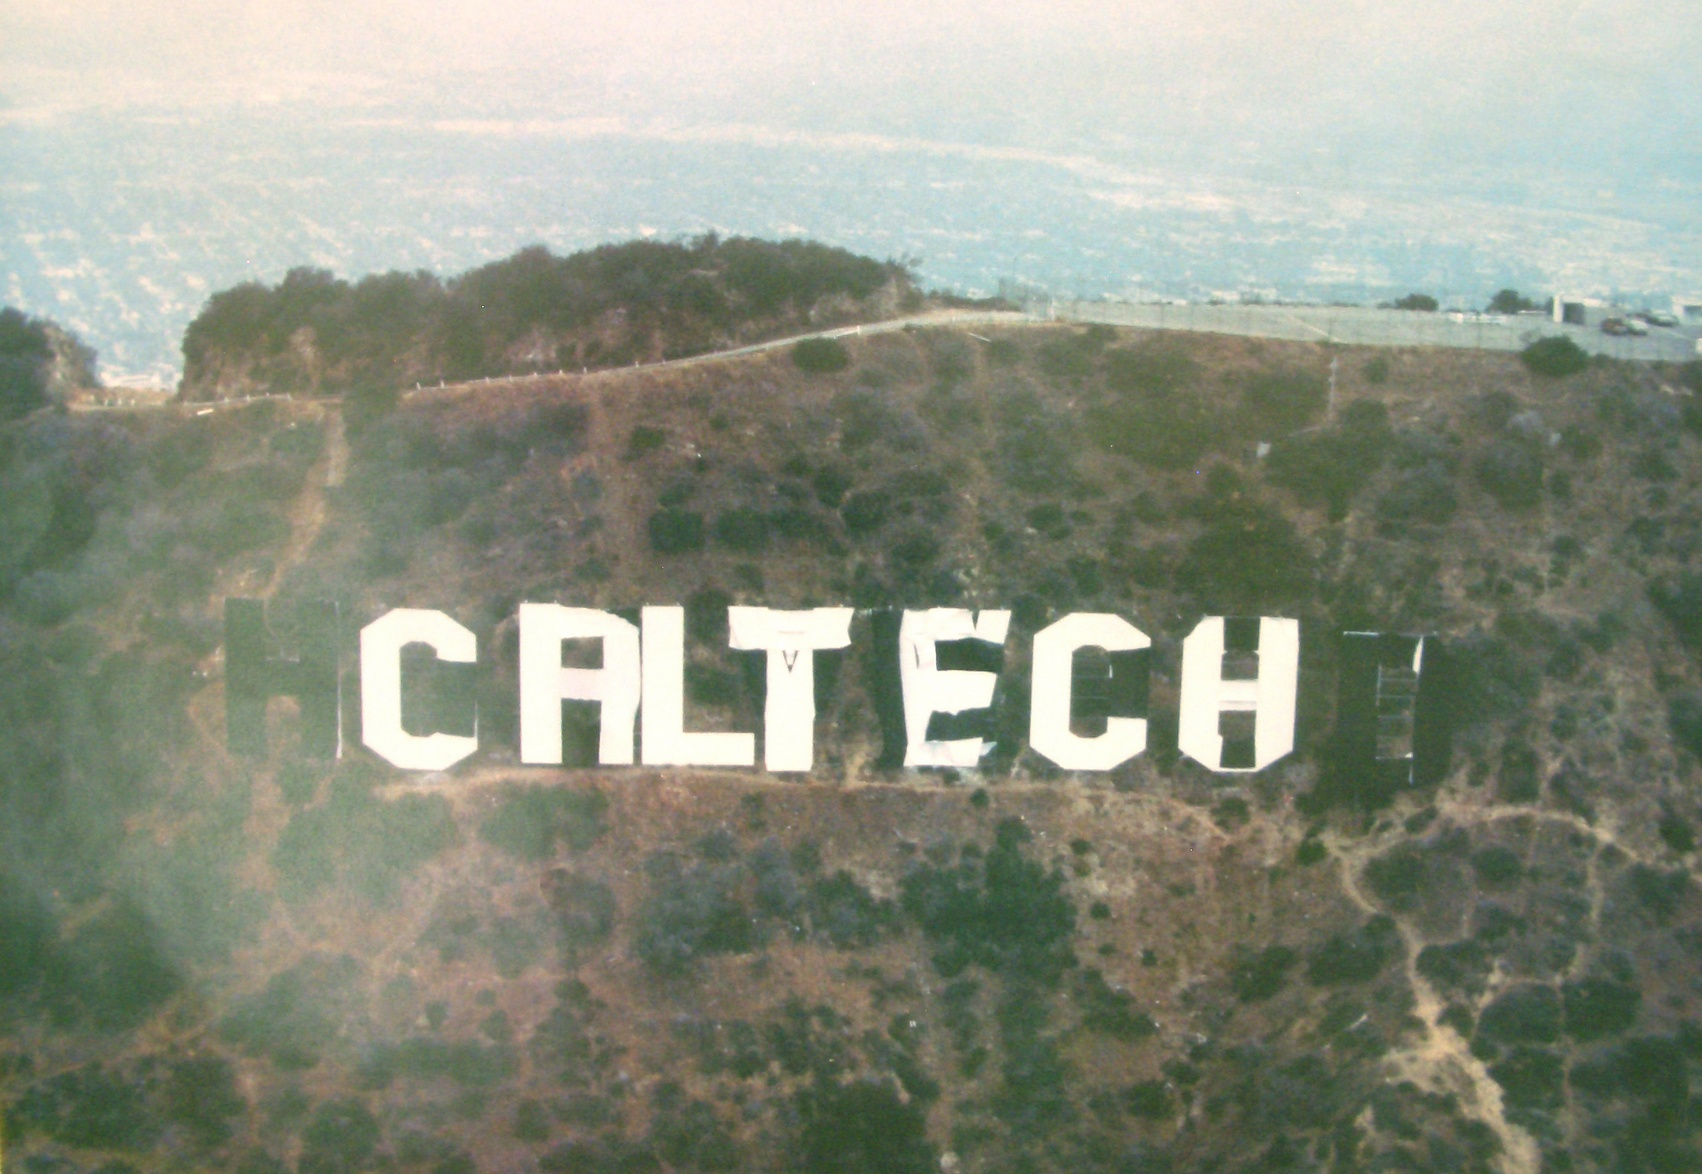
\includegraphics[width=\columnwidth]{./picture/hollywood_caltech.jpg}
    \caption{``Hollywood is still mad about that,'' says Autumn Looijen, author of \emph{Legends of Caltech III: Techer In the Dark.} \tiny{(Photo downloaded from: http://brennen.caltech.edu/autobiography/automaster2.htm)}}
    \label{fig:hollywood_prank}
\end{figure}


\column{0.55\textwidth}
In May 1987, undergraduates from Page and Ricketts houses combined forces (and several hundred dollars) to purchase enough black and white plastic, transformed the Hollywood sign to read ``Caltech''.

\small{(Reference: http://www.admissions.caltech.edu/pranks)}

\end{columns}
\end{frame}
